\chapter{For users}

\section{Installation}

The project's minimum requirement is Python, \cite{python} version 3.7 or higher.
For local testing it is recommended to use Docker \cite{docker} for running
supporting services, such as blockchain nodes and database,
along with Docker Compose utility.

After cloning sources it is recommended to create a local Python
virtual environment \cite{venv}, so as not to clutter the global installation with project's
dependencies.
All packages can be managed
using official Python package installer \texttt{pip} \cite{pip},
which comes bundled in with most Python distributions.
First, the library must be installed for local use,
and after that, the application itself.
\begin{verbatim}
    $ pip install -e lib[dev]
    $ pip install -e app[dev]
\end{verbatim}

After installation, supporting services should be set up in the background;
this can be done with \texttt{docker-compose}, i.e.:
\begin{verbatim}
    $ docker-compose up -d
\end{verbatim}

At this point, there should be a blank database available for connecting,
which needs to be populated with required tables etc.:
\begin{verbatim}
    $ flask db upgrade -d app/migrations
\end{verbatim}

What is left is to spin up a web server,
the development one bundled with Flask will do
(specify port using the flag, default is 5000):
\begin{verbatim}
    $ flask run --port 5000
\end{verbatim}

The application can be accessed from any web browser now.

\section{User guide}

\subsection{Accessing wallets}

To view a wallet, click a button in the upper-right corner of the page.

\begin{figure}[ht]
    \centering
    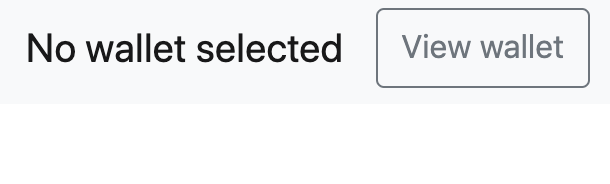
\includegraphics{assets/view-wallet.png}
    \caption{Access to wallet}
    \label{5:fig:view-wallet}
\end{figure}

You will be redirected to a page containing a form resembling
a sign-in from other web applications.
One notable difference is that private key is not required at this point,
so any wallet with known address can be viewed, not just current user's.
This might not seem very intuitive at first,
but it is designed in accordance with the very nature of the blockchain,
where all such information is public.

\begin{figure}[ht]
    \centering
    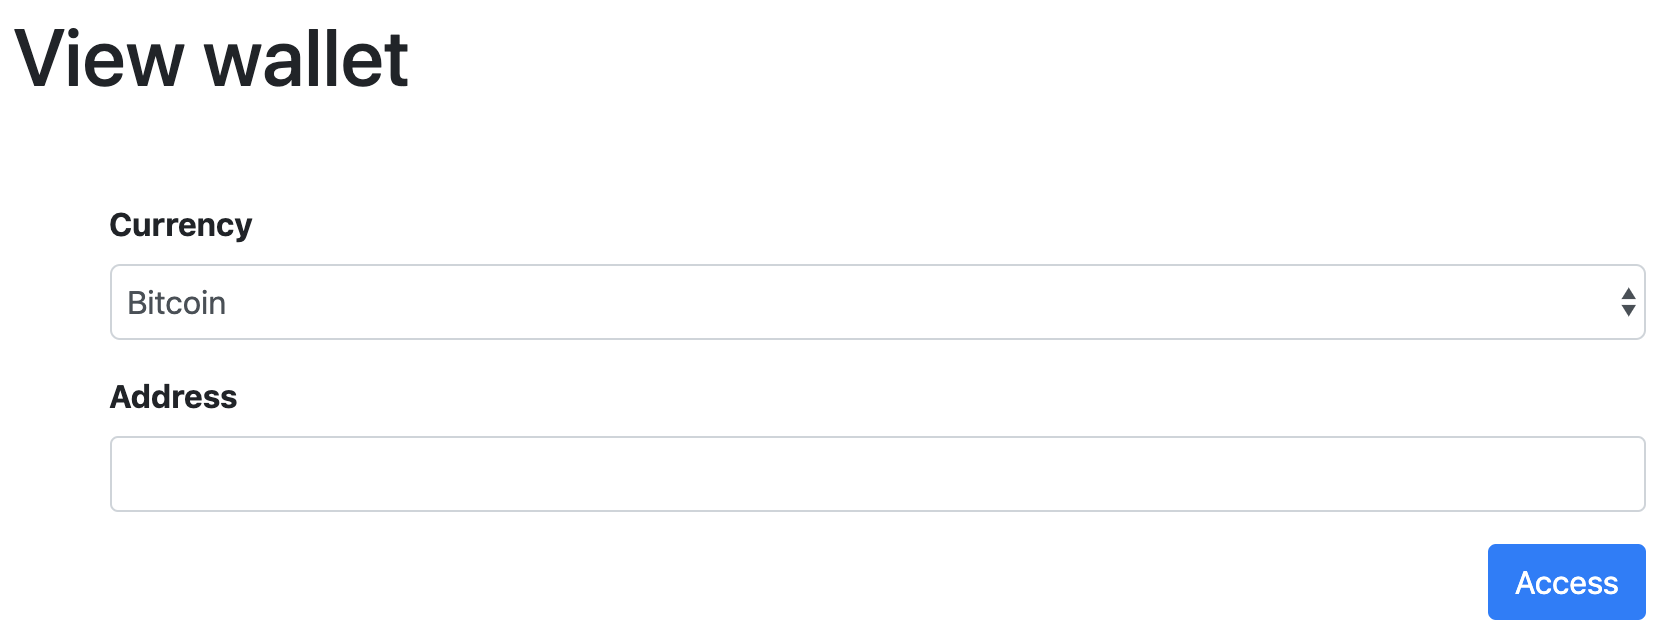
\includegraphics[width=0.7\textwidth]{assets/login.png}
    \caption{Login-like page}
    \label{5:fig:login}
\end{figure}

\newpage

\subsection{Creating or recovering wallets}

If the user doesn't have any wallet to manage yet,
they are shown an option to create a new one,
or recover one from a mnemonic phrase.
After clicking the button, they are redirected to another page
with a simple form:

\begin{figure}[ht]
    \centering
    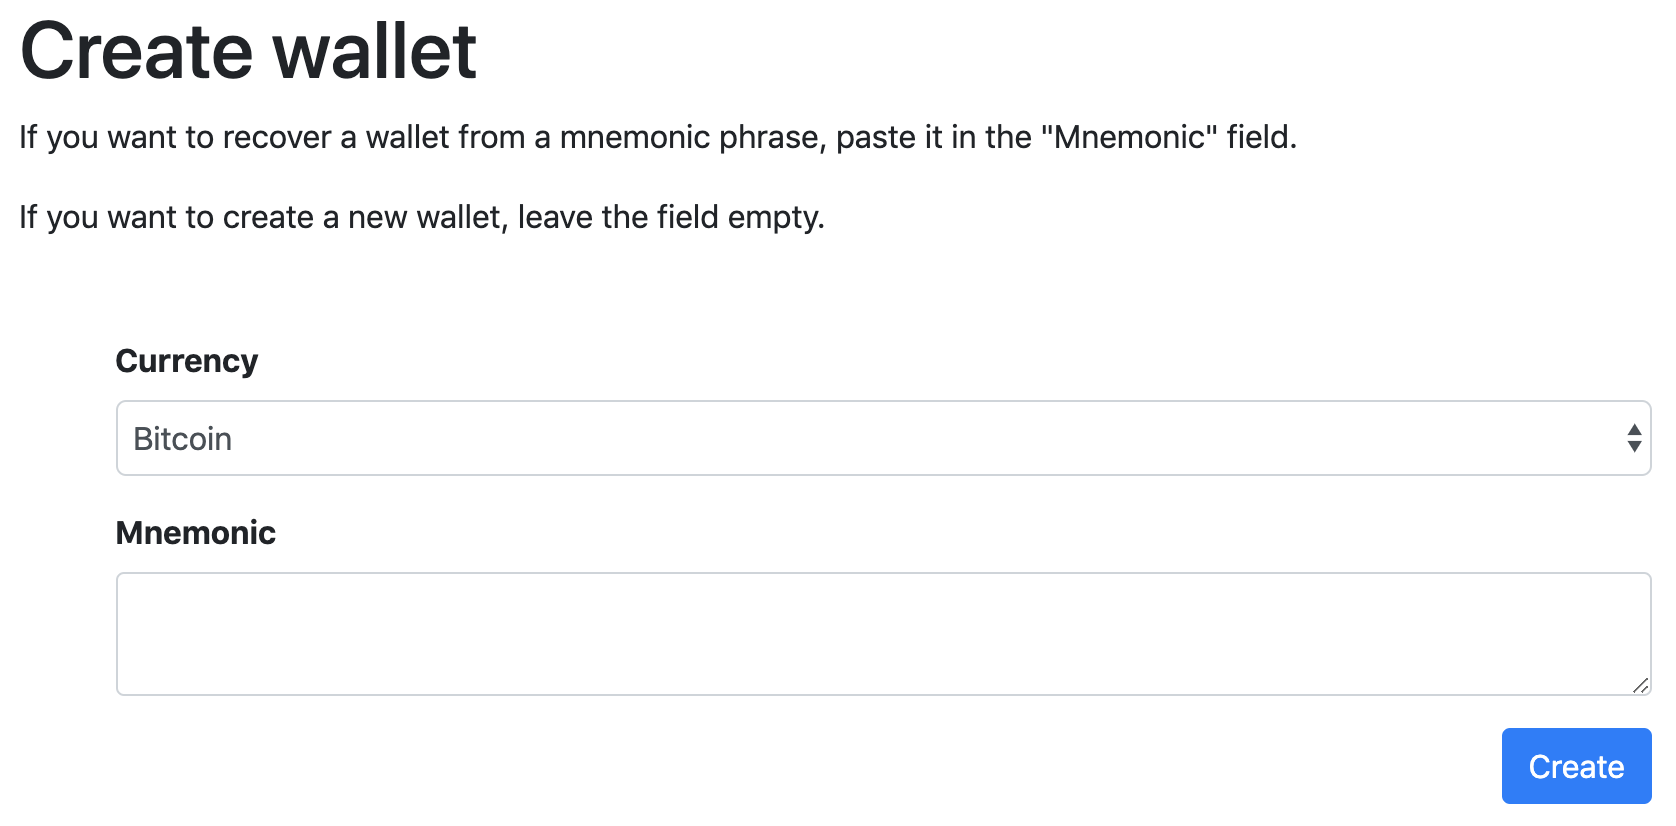
\includegraphics[width=0.7\textwidth]{assets/create-wallet.png}
    \caption{Creating a new wallet}
    \label{5:fig:create-wallet}
\end{figure}

After a successful creation of a wallet, the user is presented
with its private key and mnemonic phrase.
It's crucial to save them at this point,
because this is the last time such information will be available
(for security reasons it is not saved anywhere in the system).

\begin{figure}[ht]
    \centering
    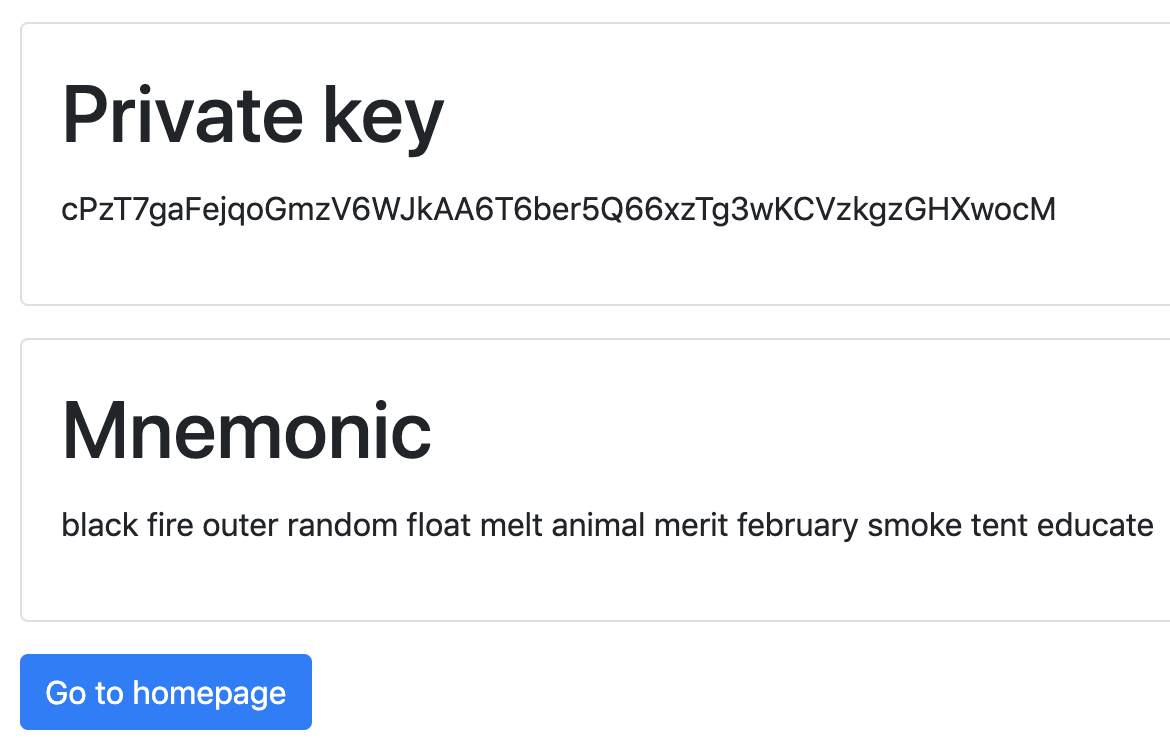
\includegraphics[width=0.7\textwidth]{assets/wallet-created.png}
    \caption{Wallet successfully created}
    \label{5:fig:wallet-created}
\end{figure}

After saving secret information, the user has an option
to be redirected to homepage in context of the newly created wallet,
as if they accessed it by its address.

\newpage

\subsection{Viewing wallets}

When using site in context of a selected address,
the user is presented with a balance over time chart and a short summary
of the funds available,
along with an option to make a transfer.

\begin{figure}[ht]
    \centering
    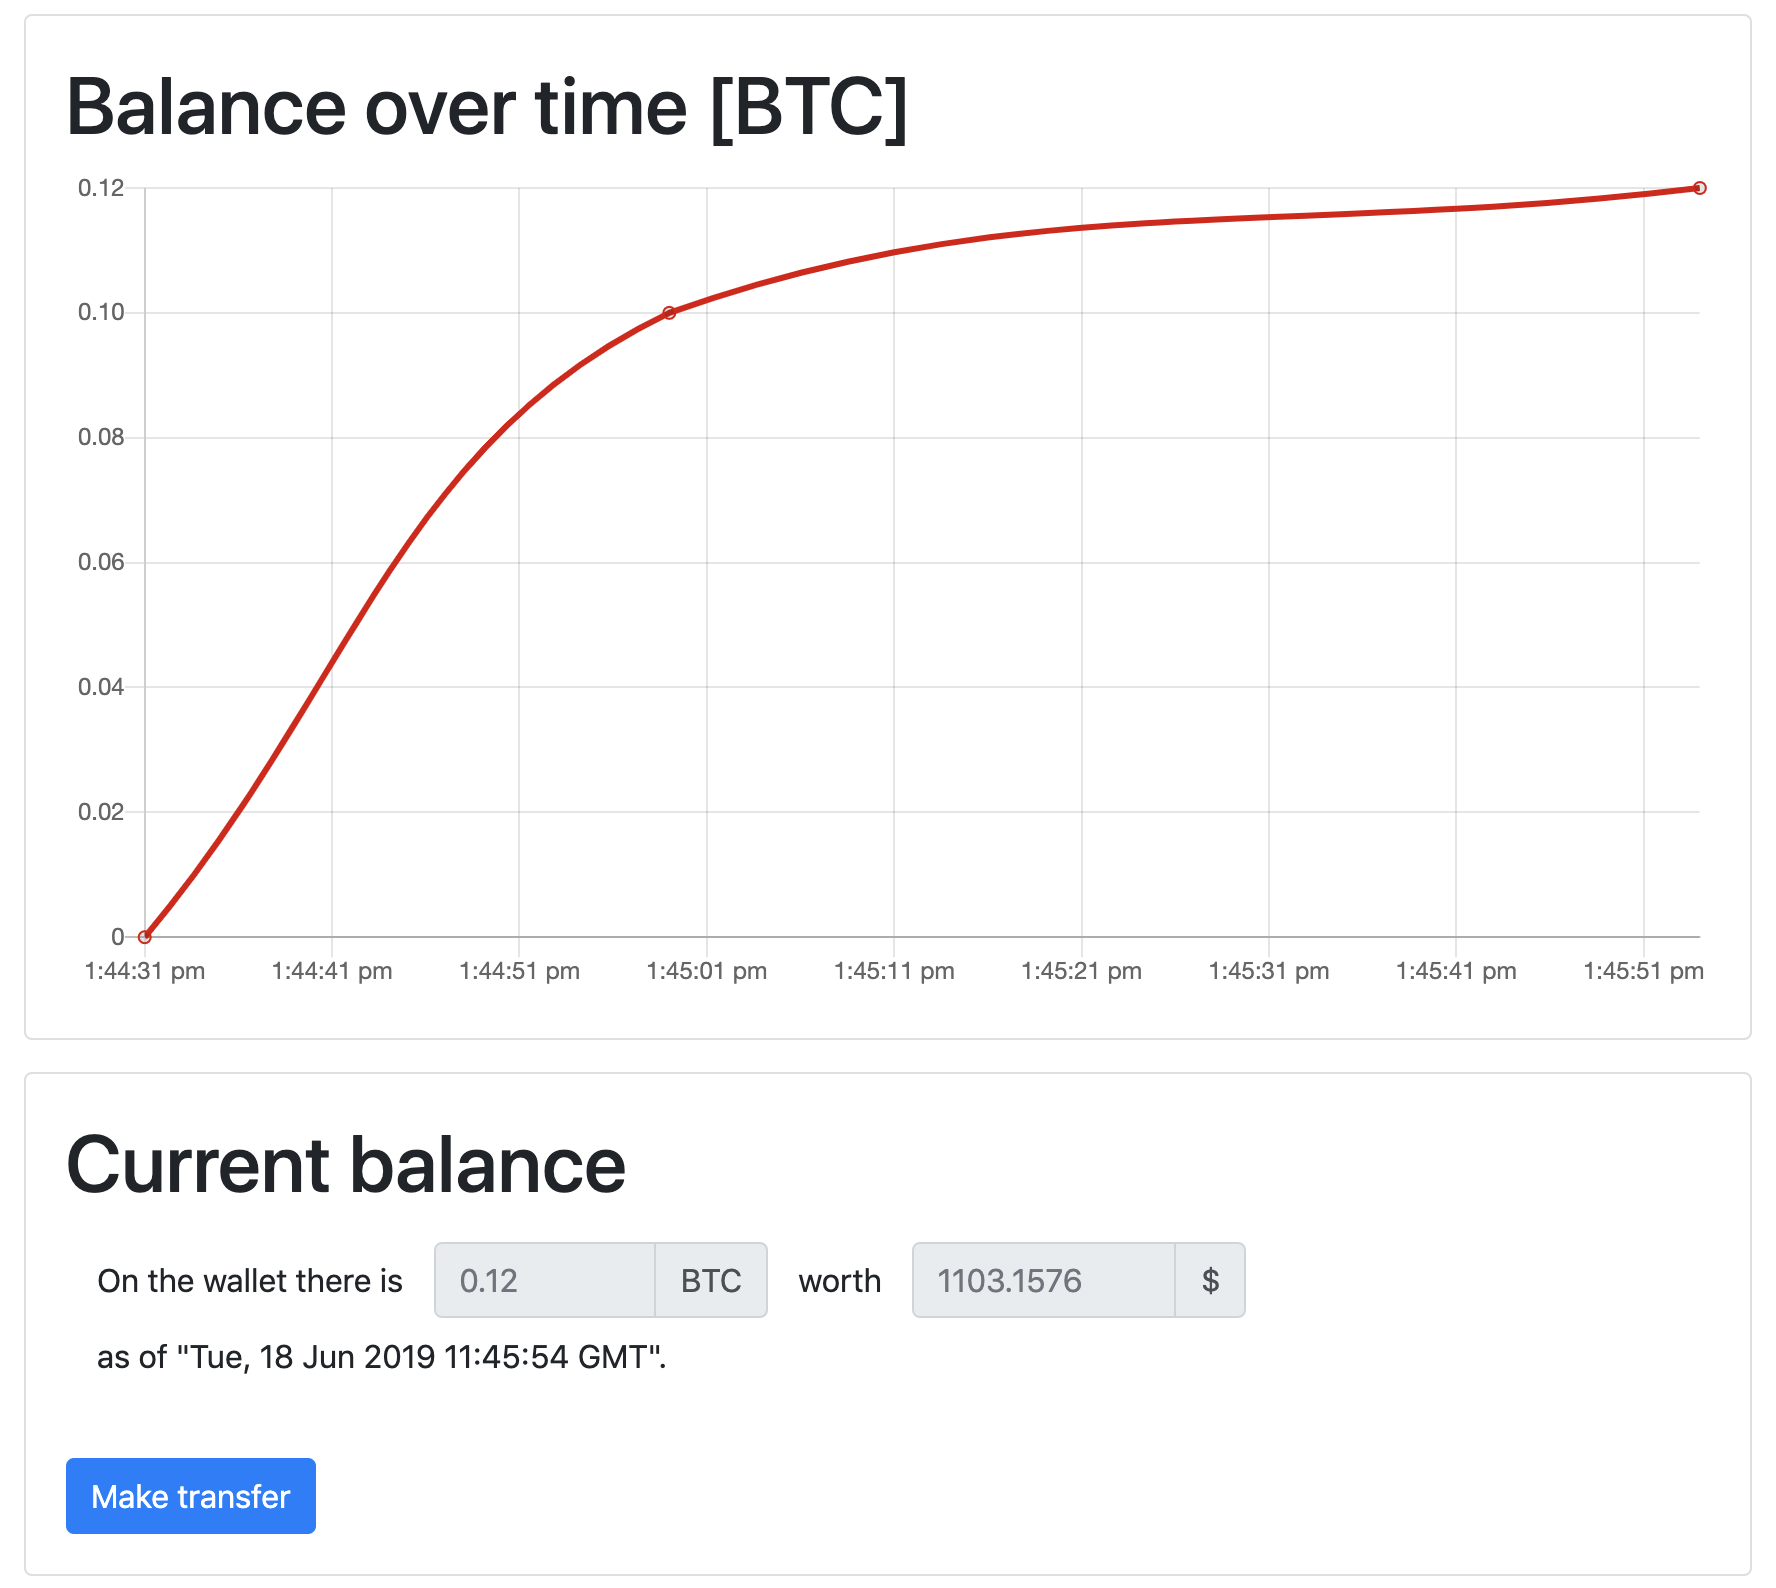
\includegraphics[width=0.7\textwidth]{assets/homepage.png}
    \caption{Homepage of a selected address}
    \label{5:fig:homepage}
\end{figure}

Below, on the same page, there is a similar chart
presenting value of the user's assets in dollars over time,
as it doesn't have to be correlated with the balance itself,
and a table providing a more detailed insight into various useful data.

During this entire time,
on all pages that current user can interact with,
they are presented with the wallet context (currency and address)
on the navigation bar.
If they wish to exit it,
the appropriate button is available in the upper-right cornet,
which is slightly similar to a logout on most websites.

\begin{figure}[ht]
    \centering
    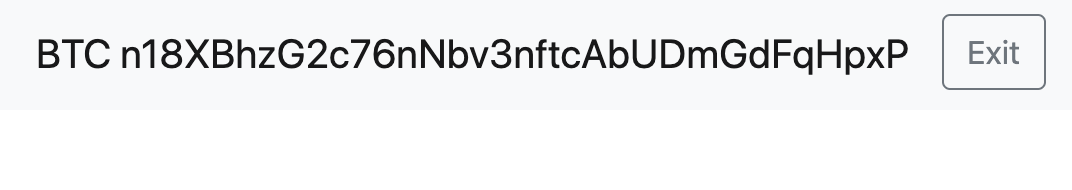
\includegraphics[width=\textwidth]{assets/logout.png}
    \caption{Wallet context}
    \label{5:fig:logout}
\end{figure}

\subsection{Making transfers}

In order to make a transfer,
the user ought to click the button described above.
After that action, they are redirected to transfers page
with a form to fill.
Desired number of recipients should be set accordingly,
and user wallet's private key must be provided for authorization.
It will be used only for this one transfer,
and will not be saved anywhere for security.
Appropriate amounts to send to their respective addresses
are to be filled in below.

\begin{figure}[ht]
    \centering
    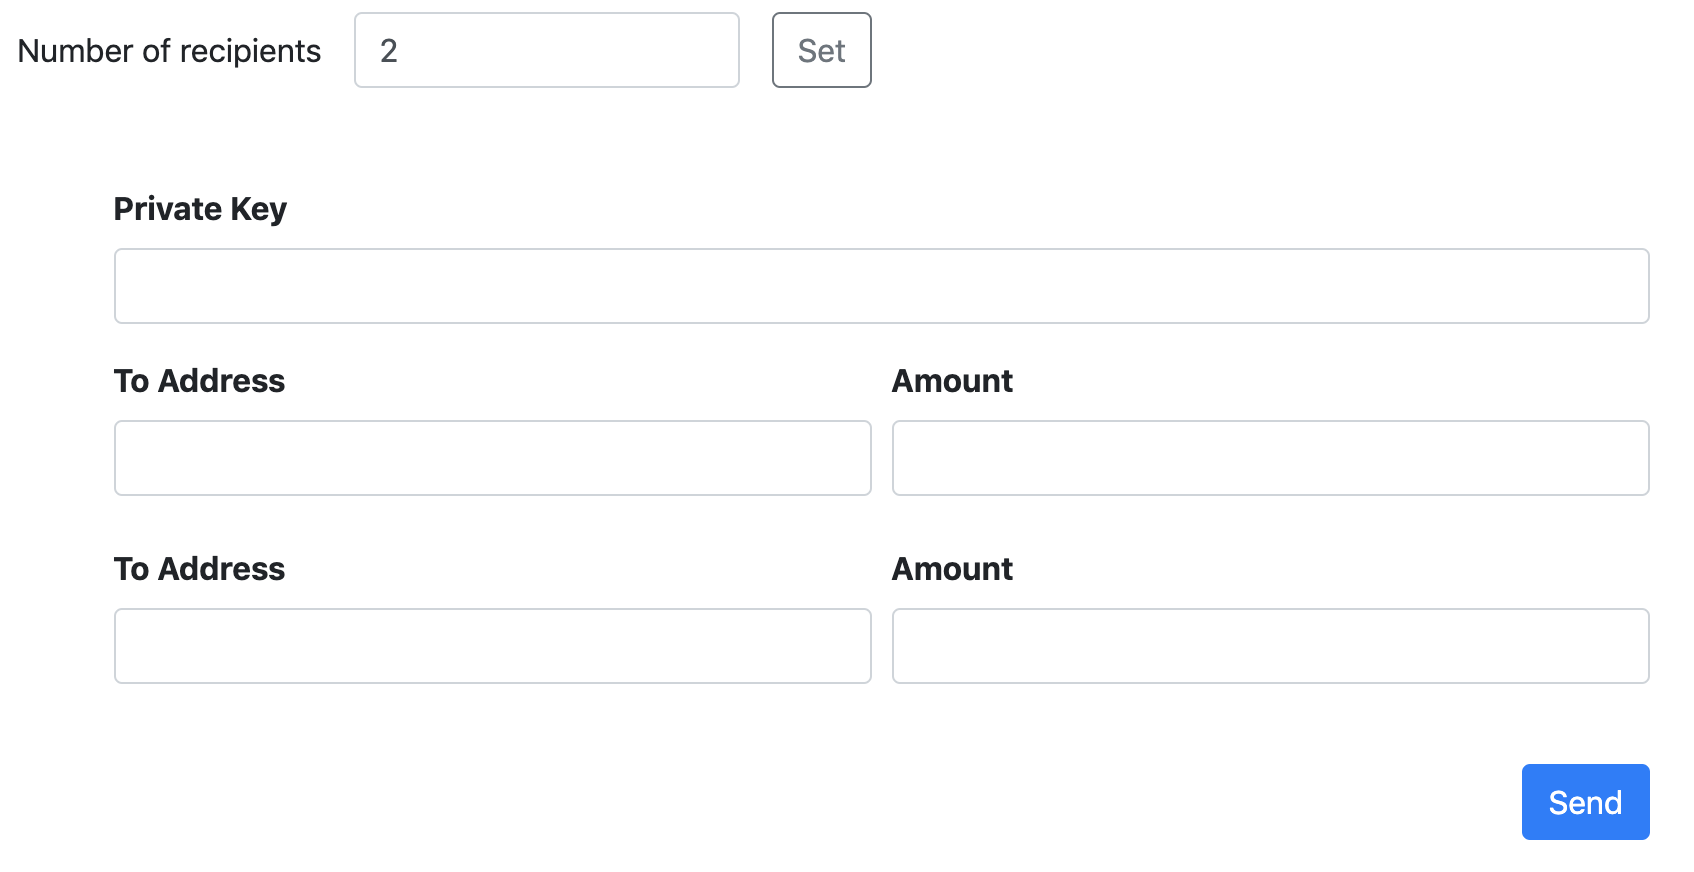
\includegraphics[width=0.7\textwidth]{assets/transfers.png}
    \caption{Transfer}
    \label{5:fig:transfers}
\end{figure}

After a successful transfer, the user will be redirected to the homepage
and provided with transaction IDs saved in the database
(only one in Bitcoin, or $n$ in case of Ethereum,
$n$ being the number of recipients).
These can be used to check transaction statuses
(e.g. numbers of confirmations)
using online blockchain explorers.
